\section{Functions and algorithms}

\begin{frame}
\frametitle{Incomplete list of OTB functions}

\begin{block}{Pre-processing}
\begin{itemize}
\item Radiometric calibration, orthorectification, resampling (raster and
  vector), pan-sharpening, stereo rectification\ldots
\item Sensor supported: Sentinels, Pléiades, SPOT6, SPOT5, Digital Globe satellites
\item Geometric models (thanks to OSSIM), support for DEM (SRTM or GeoTIFF)
\end{itemize}
\end{block}

\begin{block}{Images and vector manipulation}
\begin{itemize}
\item Formats supported by GDAL (raster and vector), conversion raster/vector
\item Region of interest extraction, of spectral bands, concatenation or splitting\ldots
\item Band math, color mapping, contrast enhancement
\item Linear filtering, Mathematical morphology
\end{itemize}
\end{block}
\end{frame}

\begin{frame}
\frametitle{(Incomplete) List of OTB functions}

\begin{block}{Feature extraction}
\begin{itemize}
\item Edge detection, scale-invariant feature transform, lines, corners
\item Radiometric indices, textures (Haralick, SFS, PanTex)
\item Local statistics (Flusser moments, Histogram of Oriented Gradient)
\item Keypoints matching (SIFT, SURF\ldots)
\end{itemize}
\end{block}

\begin{block}{Change detection}
\begin{itemize}
\item Classic methods with image metrics comparison
\item Multivariate Alteration Detector
\end{itemize}
\end{block}

\begin{block}{Dimensionality reduction, hyperspectral processing}
\begin{itemize}
\item PCA, NAPCA, ICA, MAF\ldots
\item Dimension estimation, endmembers extraction, Vertex Component Analysis(VCA)
\end{itemize}
\end{block}

\end{frame}

\begin{frame}
\frametitle{Incomplete list of OTB functions}
\begin{block}{Segmentation}
\begin{itemize}
\item Segmentation algorithms: Connected Components, MeanShift,Watershed\ldots
\item Methods to apply those algorithms on large dataset
\item Vector or raster representation which allow Object Based Image Analysis
\end{itemize}
\end{block}

\begin{block}{Classification}
\begin{itemize}
\item 9 supervised methods available (including SVM and Random Forests)
\item Fusion and regularization of classifications
\item K-Means clustering or Kohonen maps
\item Object classification (from a segmentation)
\end{itemize}
\end{block}

\end{frame}


\vspace*{-6.5mm}
\begin{frame}[plain]
\hspace*{-11mm}
    \includegraphics[keepaspectratio,height=1.1\paperheight]{../OTB-General/images/mayotte2012.png}
\end{frame}

\vspace*{-6.5mm}
\begin{frame}[plain]
\hspace*{-11mm}
    \includegraphics[keepaspectratio,height=1.1\paperheight]{../OTB-General/images/mayotte2013.png}
\end{frame}

\vspace*{-6.5mm}
\begin{frame}[plain]
\hspace*{-11mm}
    \includegraphics[keepaspectratio,height=1.1\paperheight]{../OTB-General/images/mayotte_mad.png}
\end{frame}

\vspace*{-6.5mm}
\begin{frame}[plain]
\hspace*{-11mm}
\includegraphics[keepaspectratio,height=1.1\paperheight]{../OTB-General/images/saint_paul_lsd.png}
\end{frame}

\vspace*{-6.5mm}
\begin{frame}[plain]
\hspace*{-11mm}
    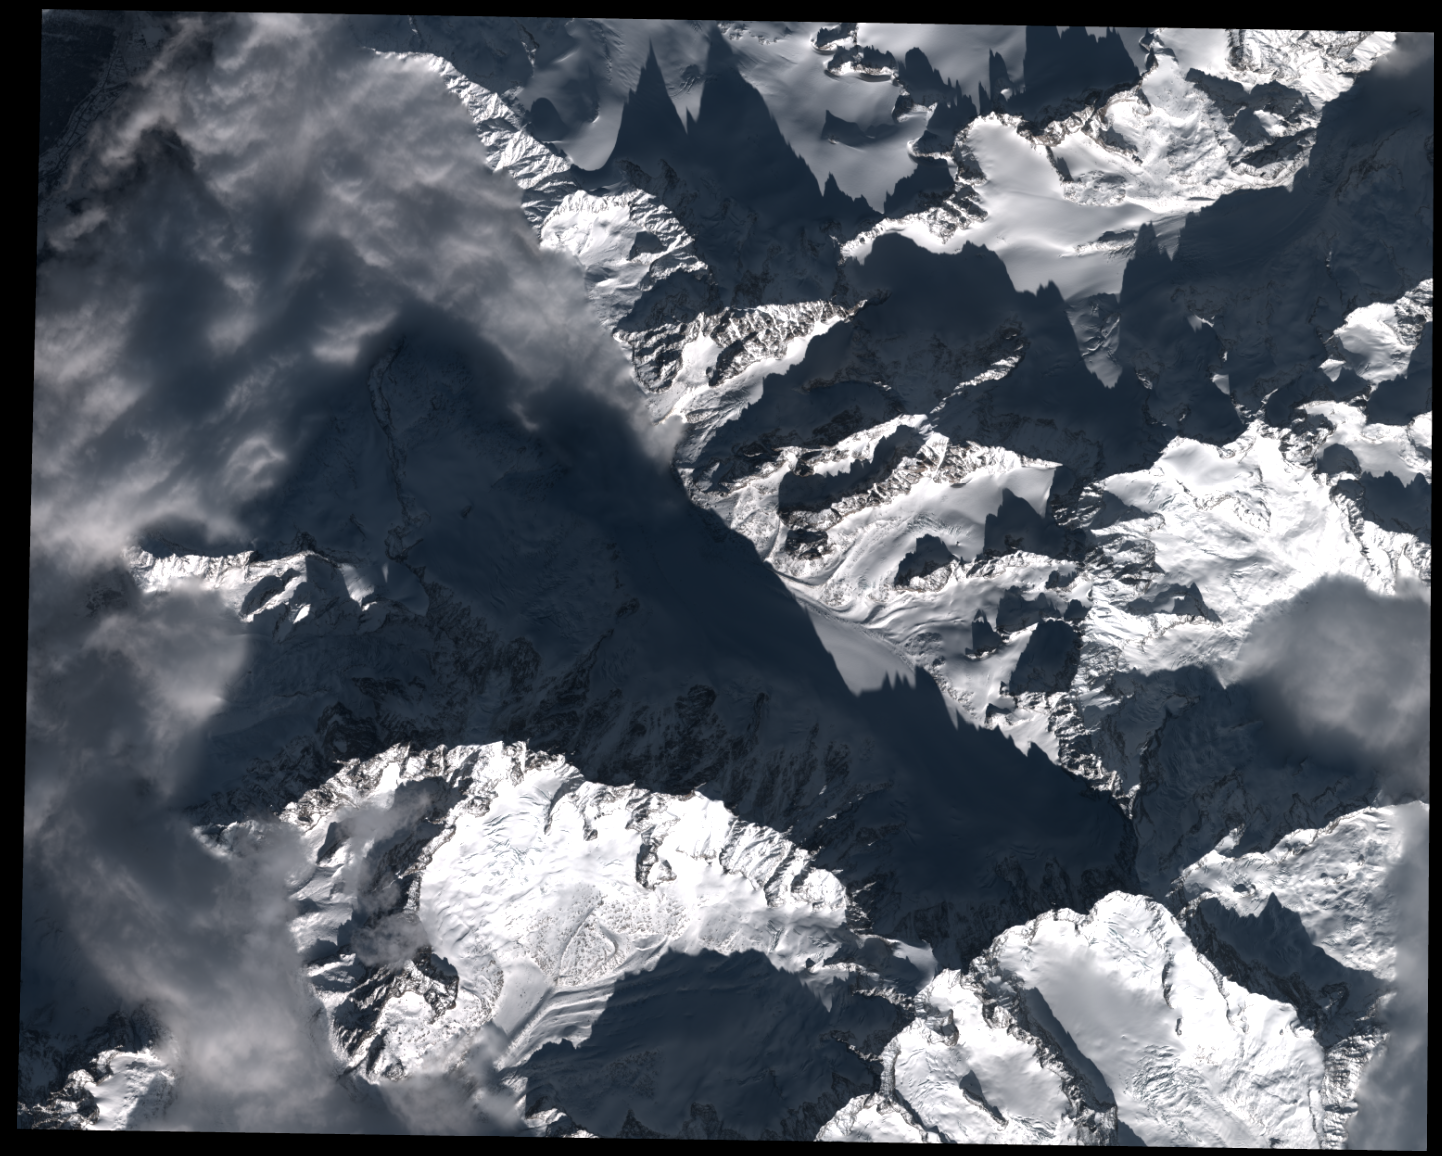
\includegraphics[keepaspectratio,width=1.005\paperwidth,height=1.1\paperheight]{../OTB-General/images/argentiere_left.png}
\end{frame}

\vspace*{-6.5mm}
\begin{frame}[plain]
\hspace*{-11mm}
    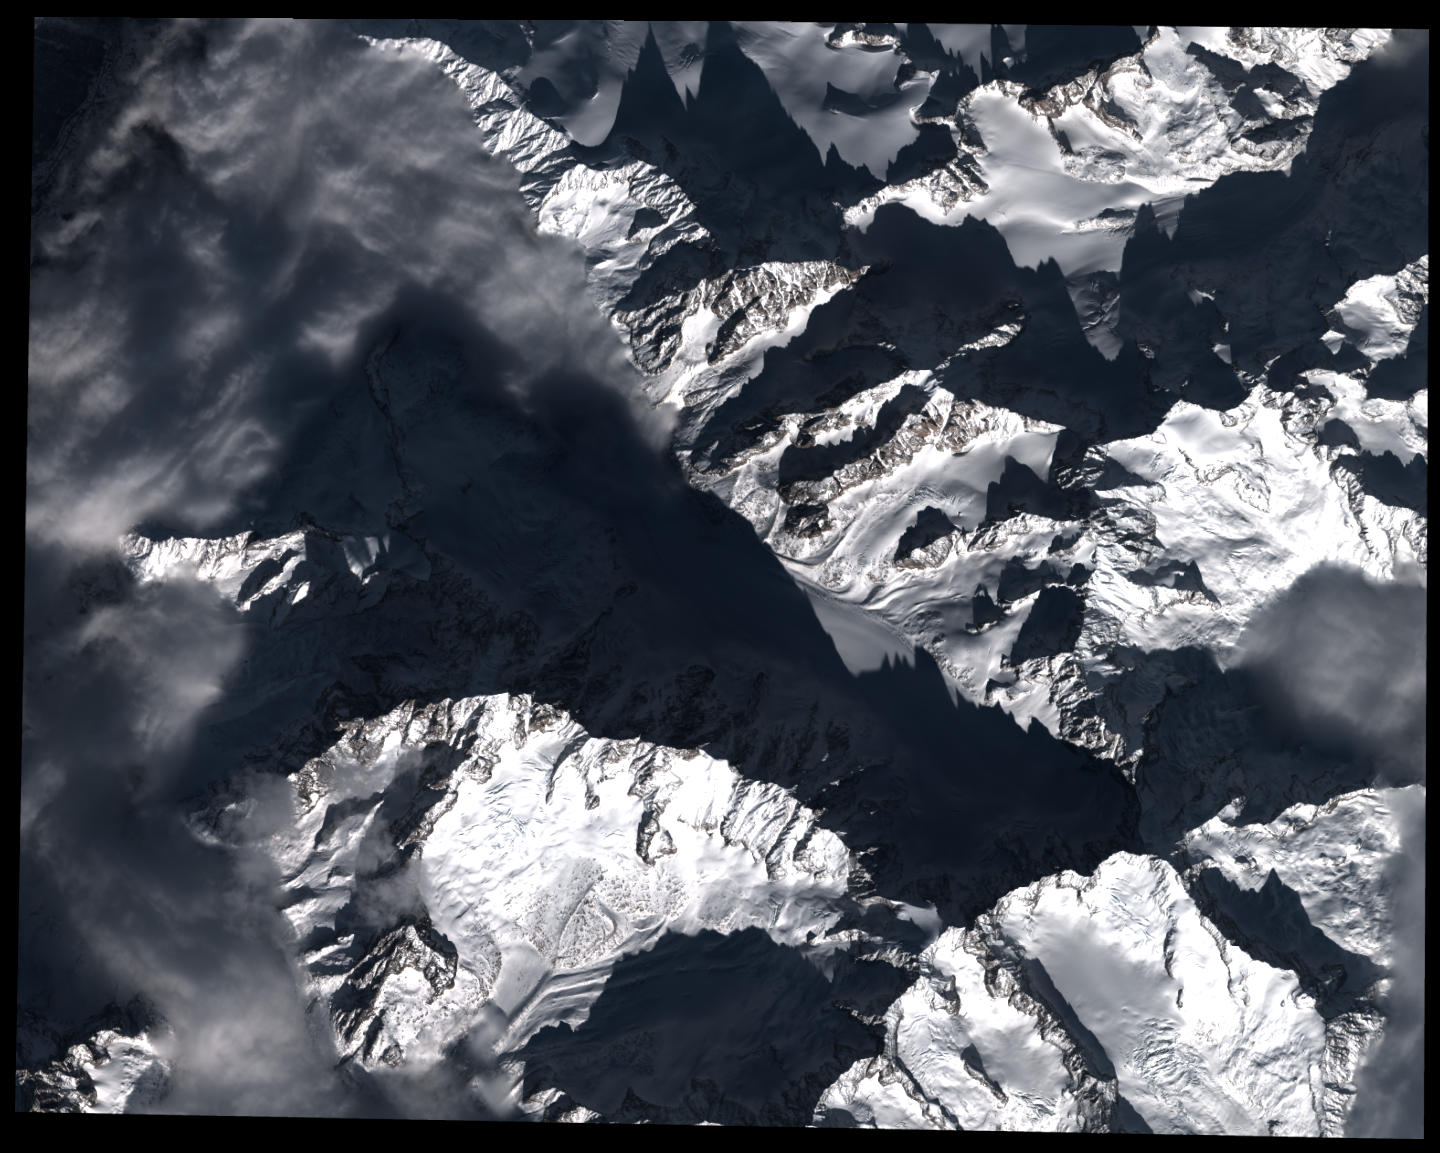
\includegraphics[keepaspectratio,width=1.005\paperwidth,height=1.1\paperheight]{../OTB-General/images/argentiere_right.png}
\end{frame}

\vspace*{-6.5mm}
\begin{frame}[plain]
\hspace*{-11mm}
    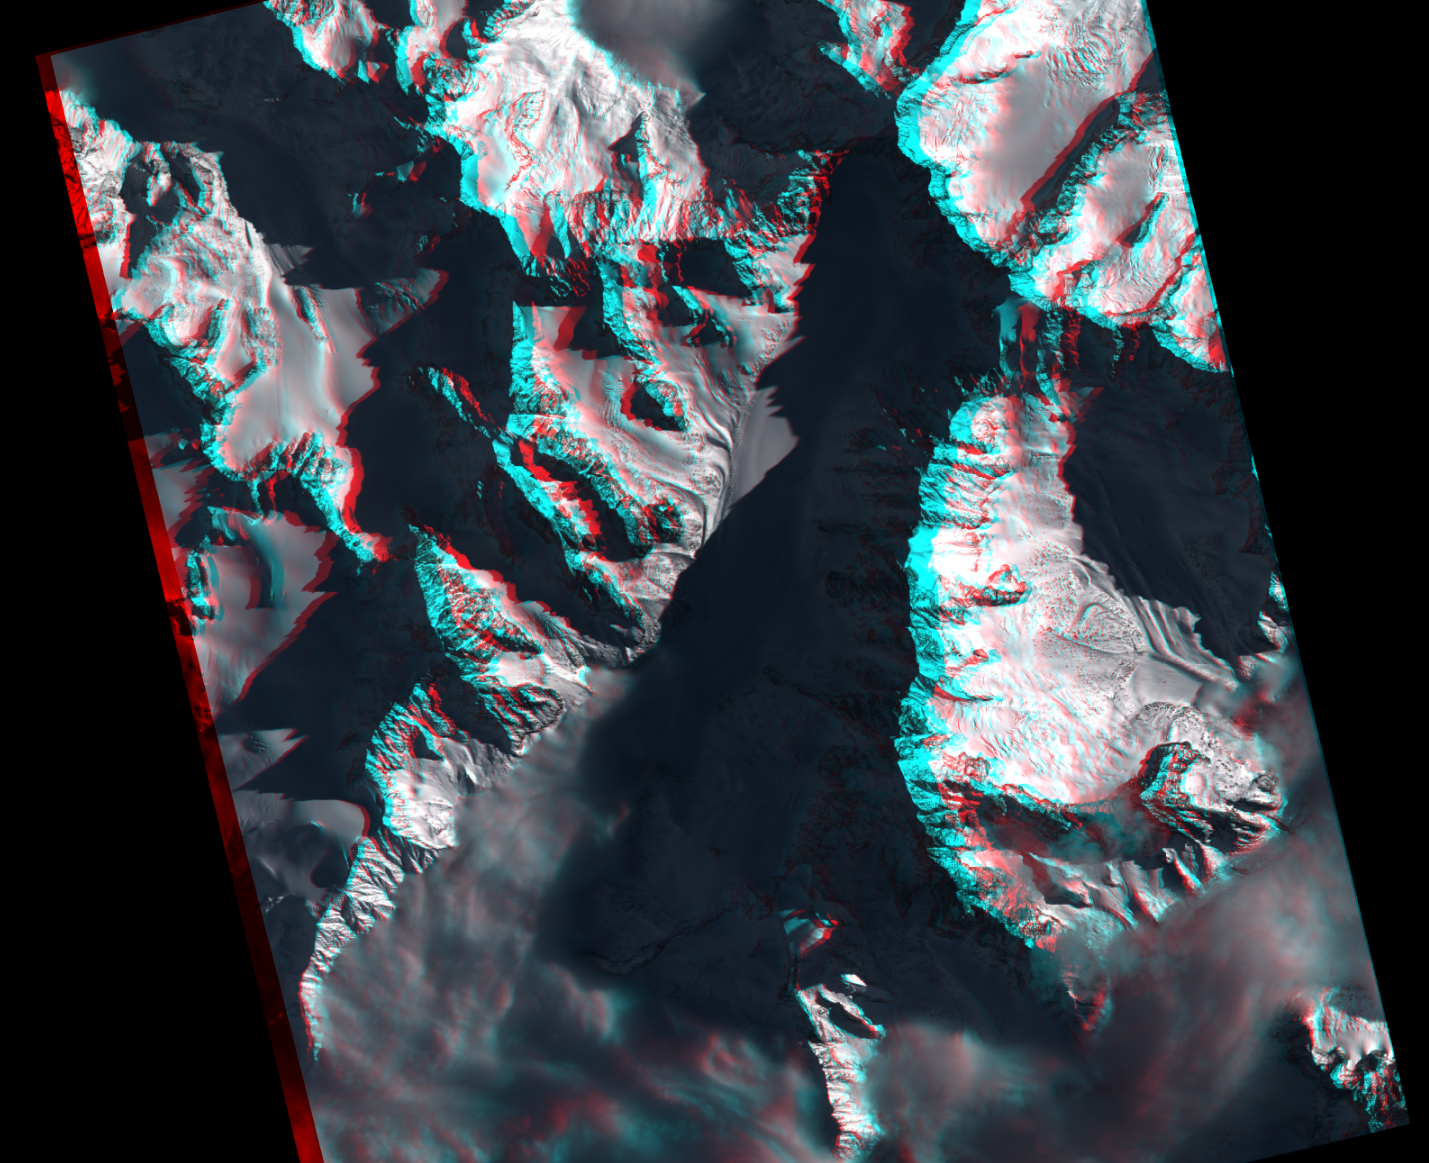
\includegraphics[keepaspectratio,width=1.005\paperwidth,height=1.1\paperheight]{../OTB-General/images/argentiere_anaglyphe.png}
\end{frame}


\vspace*{-6.5mm}
\begin{frame}[plain]
\hspace*{-11mm}
    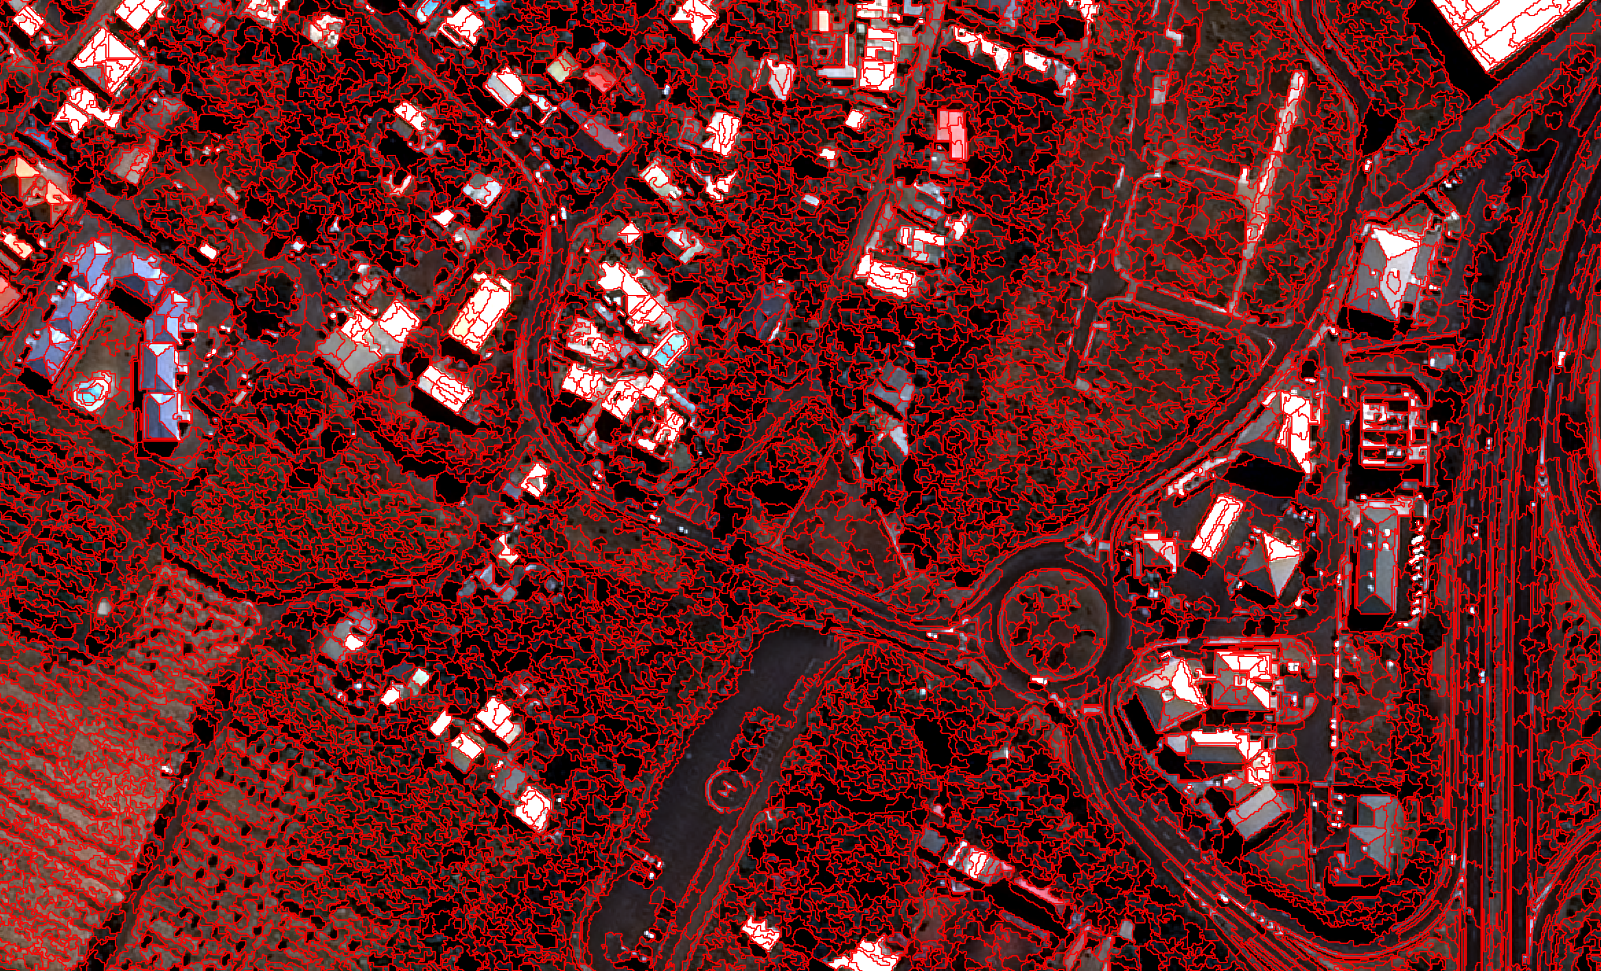
\includegraphics[keepaspectratio,height=1.1\paperheight]{../OTB-General/images/segmentation.png}
\end{frame}

\vspace*{-6.5mm}
\begin{frame}[plain]
\hspace*{-11mm}
    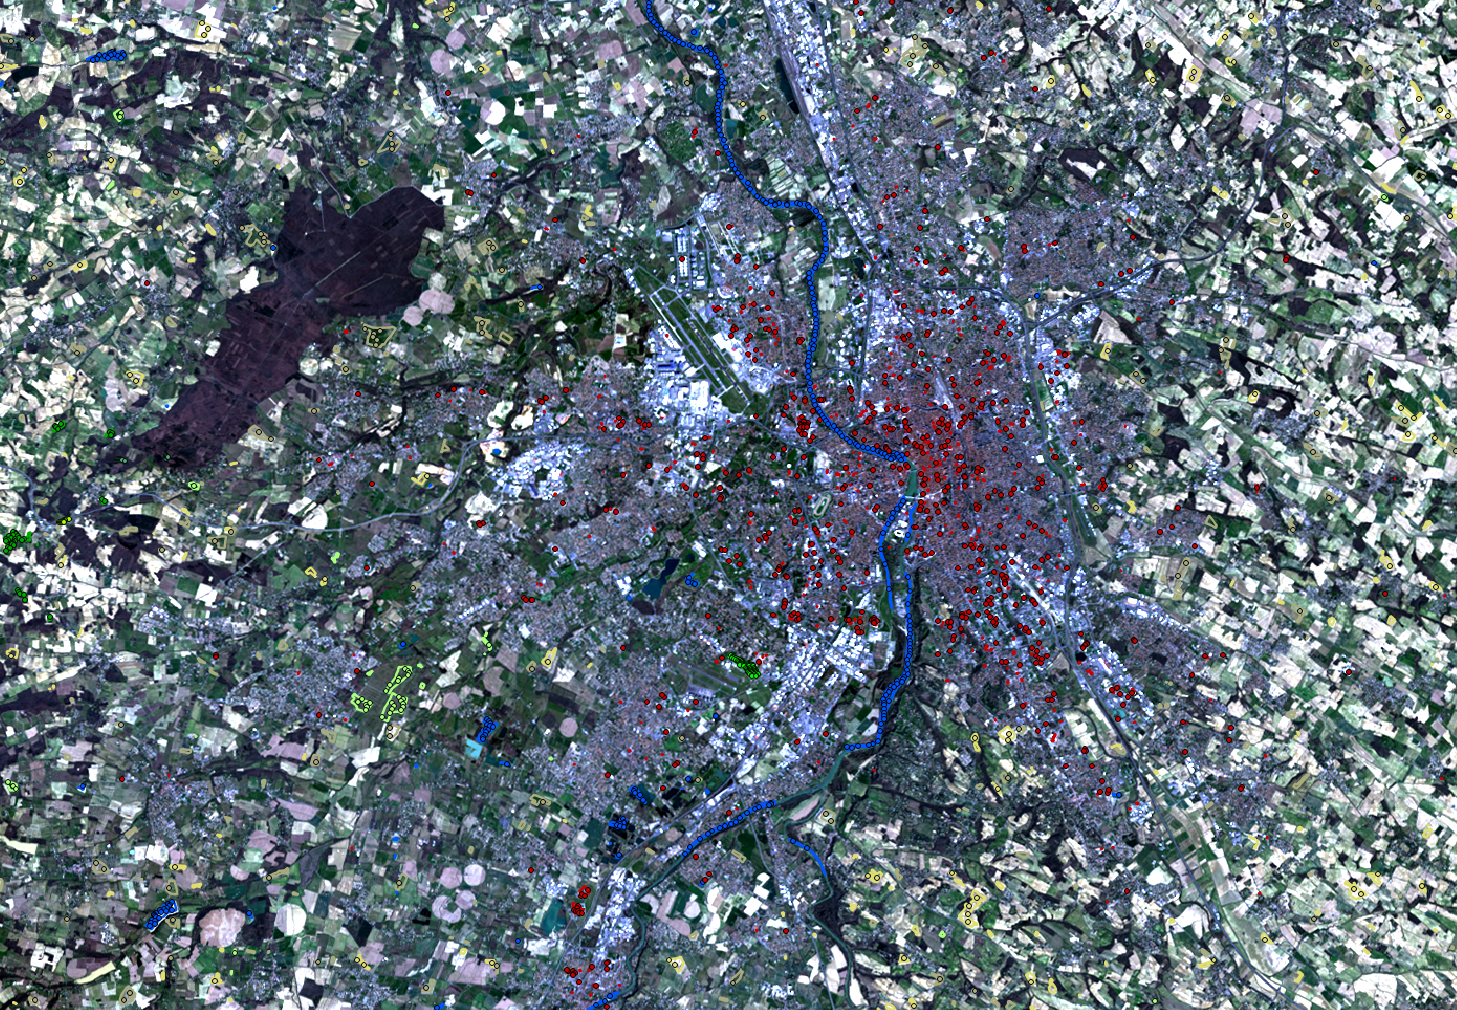
\includegraphics[keepaspectratio,height=1.1\paperheight]{../../Courses/org/WorkshopGuide/Images/samples_selection.png}
\end{frame}


\vspace*{-6.5mm}
\begin{frame}[plain]
\hspace*{-11mm}
    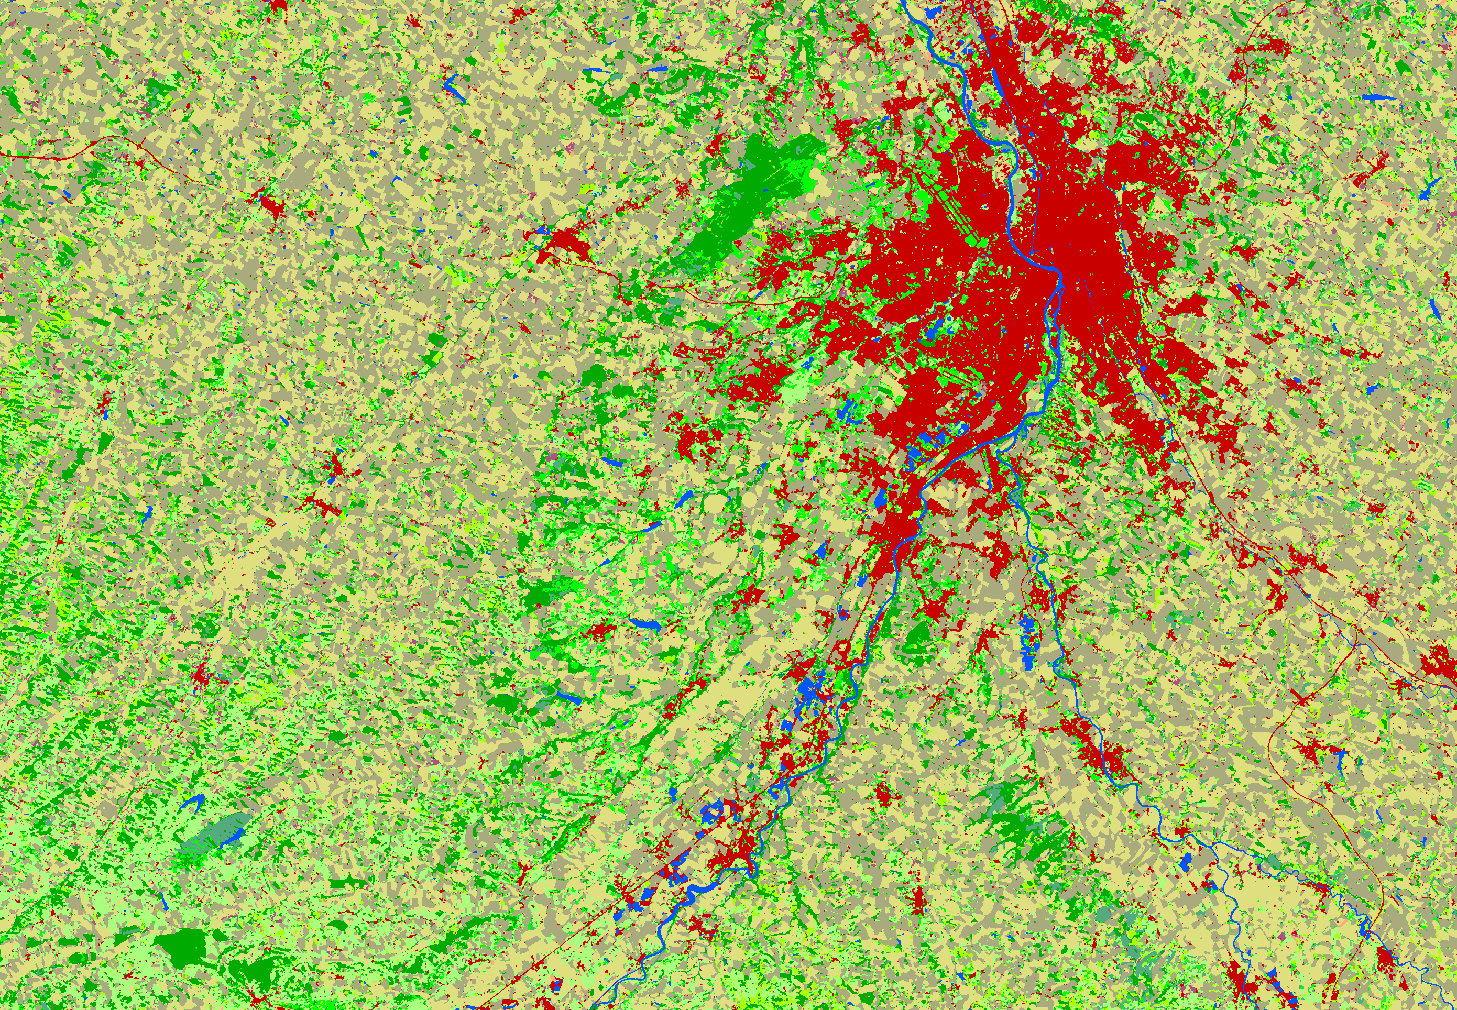
\includegraphics[keepaspectratio,height=1.1\paperheight]{../../Courses/org/WorkshopGuide/Images/final_classification.png}
\end{frame}

\vspace*{-6.5mm}
\begin{frame}[plain]
\hspace*{-11mm}
    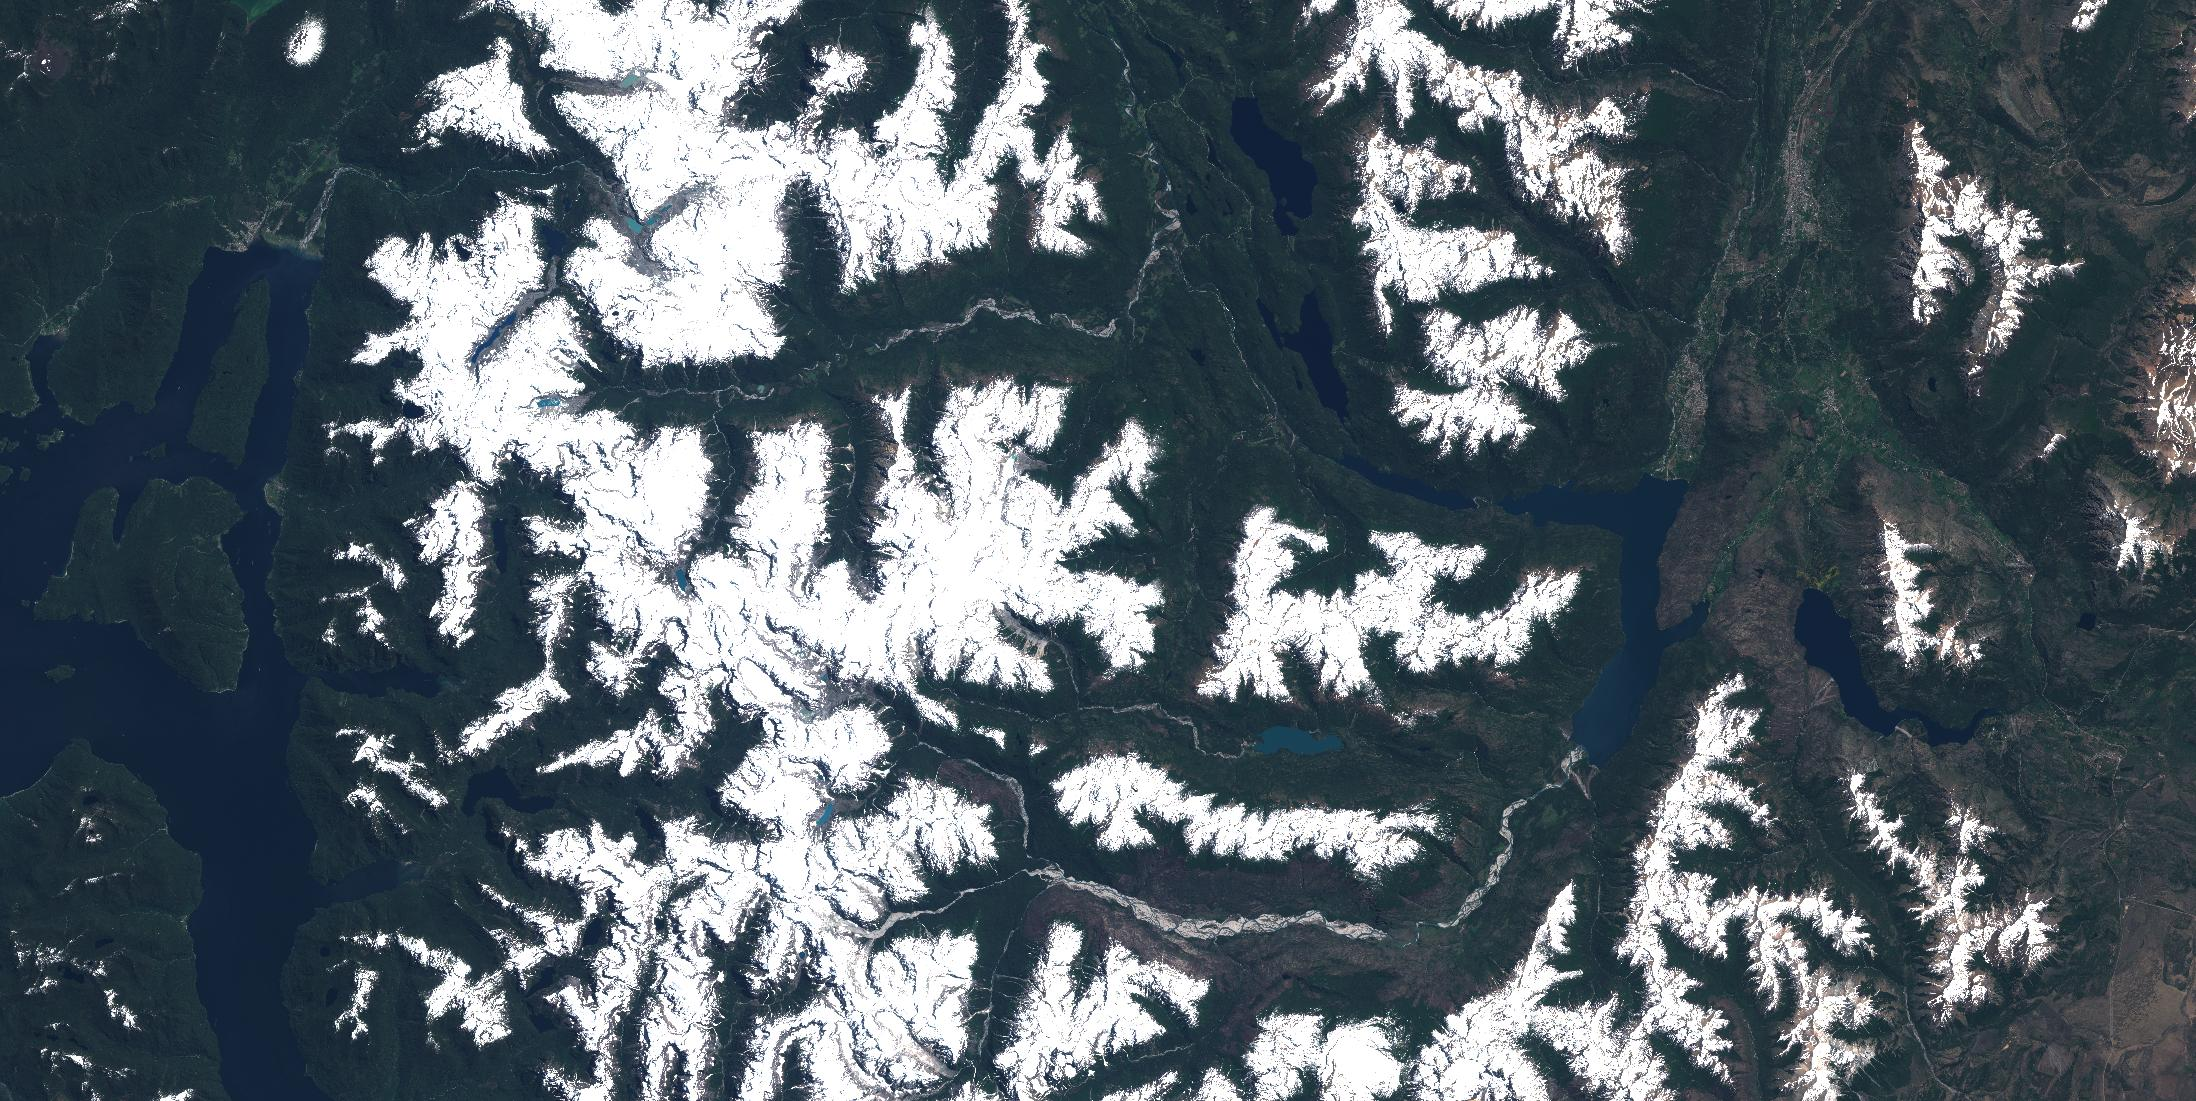
\includegraphics[keepaspectratio,height=1.1\paperheight]{../OTB-General/images/imag4tci.jpg}
\end{frame}

\vspace*{-6.5mm}
\begin{frame}[plain]
\hspace*{-11mm}
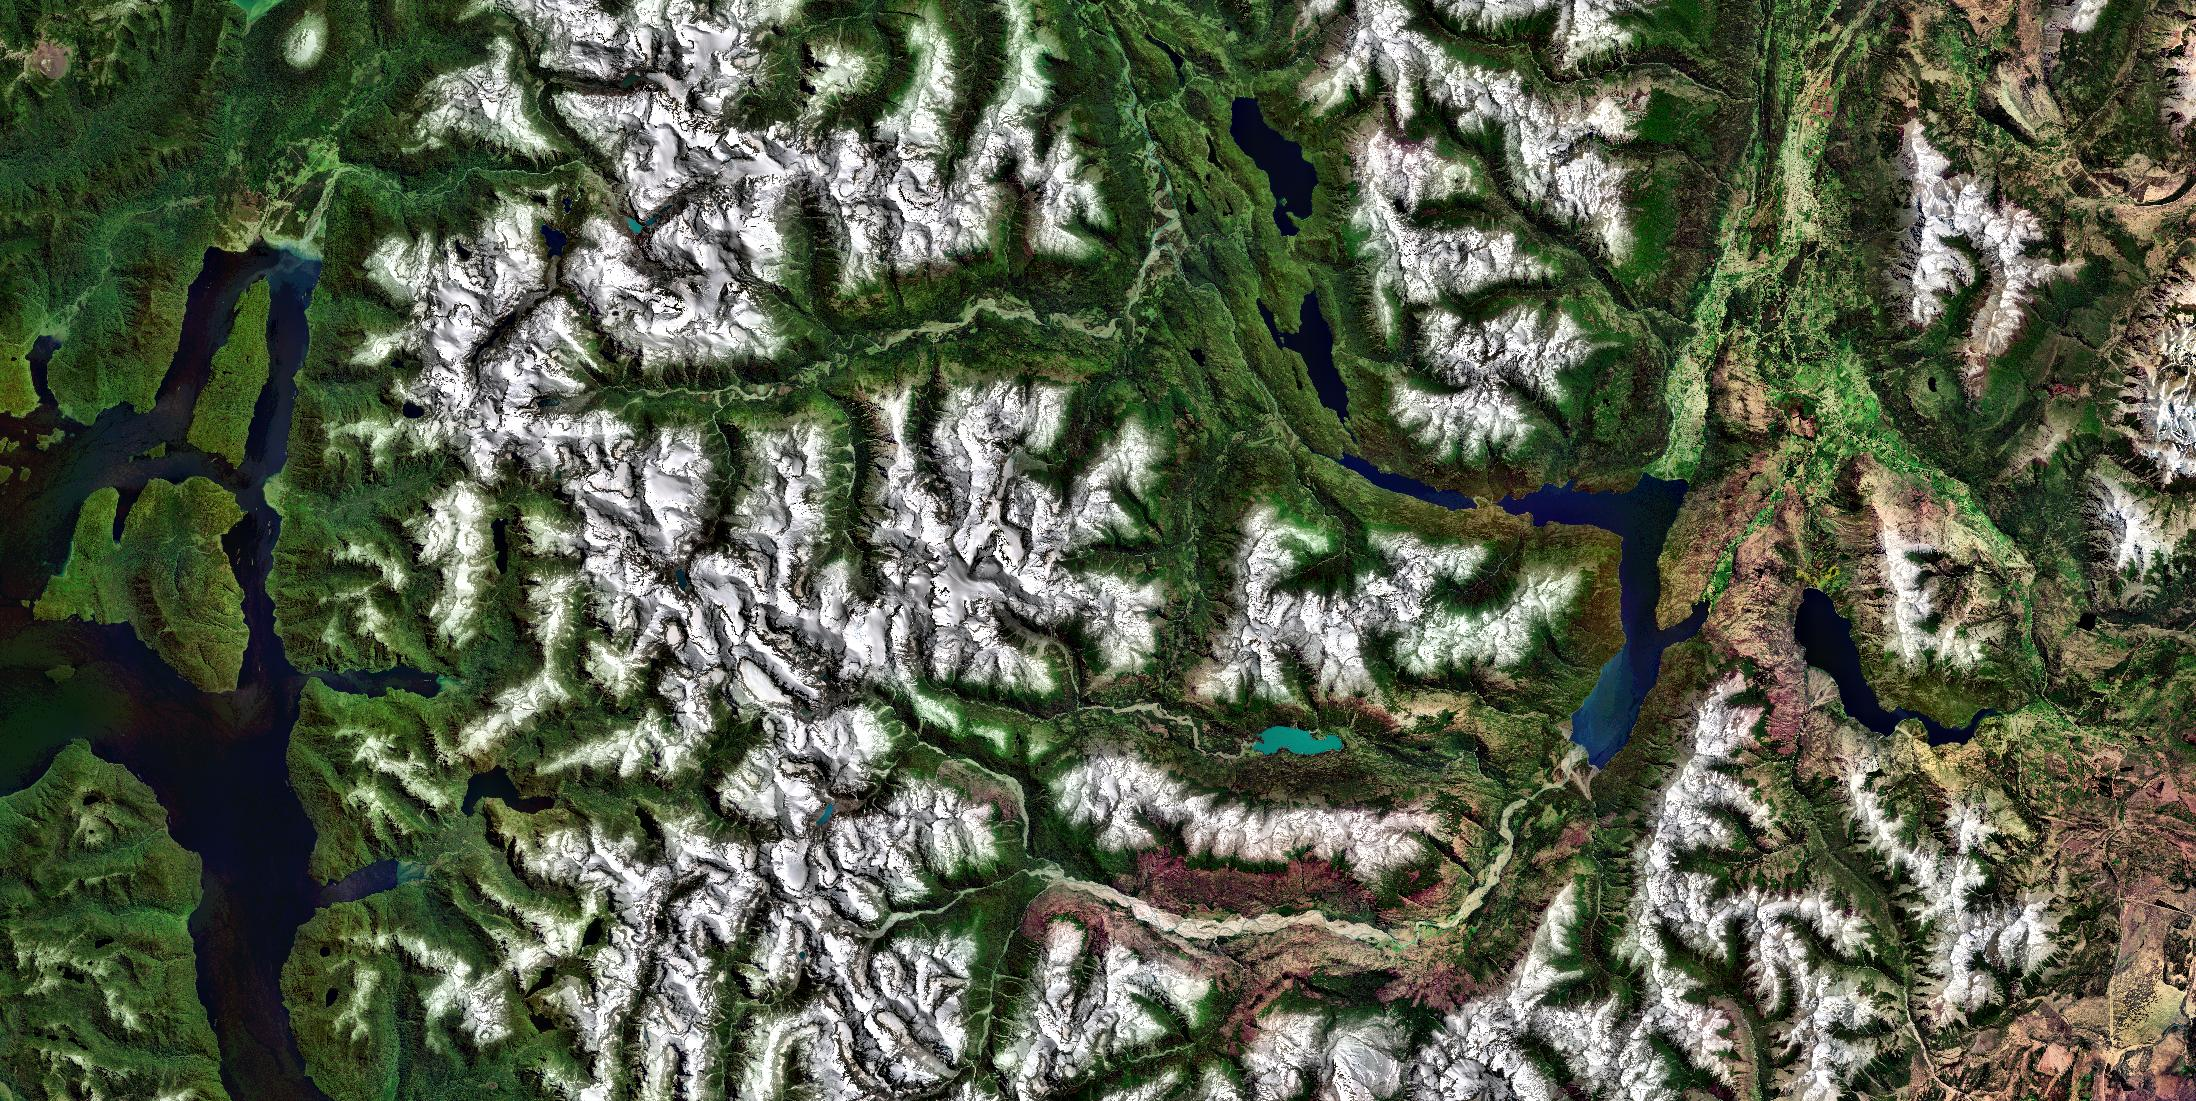
\includegraphics[keepaspectratio,height=1.1\paperheight]{../OTB-General/images/image4_glob_each_lim20_8b_sub.jpg}
\end{frame}

